
\begin{figure}[ht]
\begin{center}
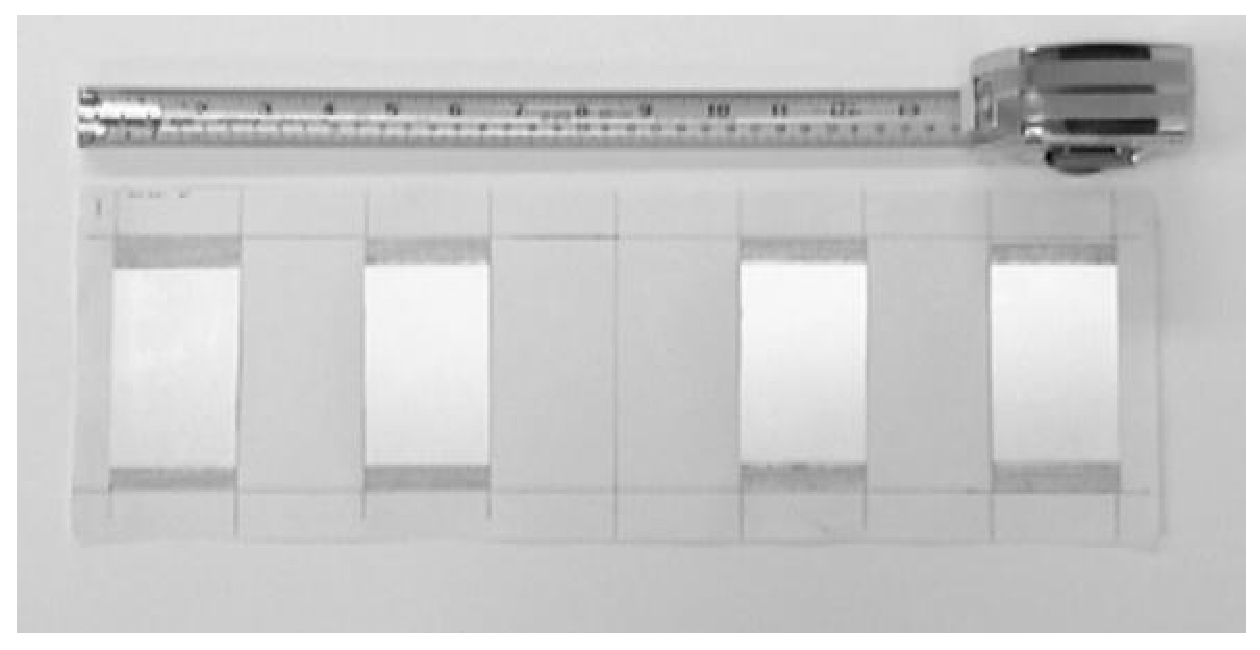
\epsfig{file=beacon.eps, height=40mm}
\caption{A sample laser barcode.  This barcode has 8 bits, each of which 
is 50mm wide.}
\label{fig:laserbarcode}
\end{center}
\end{figure}

\subsection*{Synopsis}

The laser barcode detector searches for specially constructed barcodes
in the laser range finder data.  An example laser barcode is shown in
Figure \ref{fig:laserbarcode}.  The barcode is constructed using
strips of retro-reflective paper.  Each retro-reflective strip
represents a `1' bit; each non-reflective strip represents a `0' bit.
By default, the {\tt laserbarcode} driver searches for barcodes
containing 8 bits, each of which is exactly 50mm wide (the total
barcode width is thus 400m).  The first and last bits are used as
start and end markers, and the remaining bits are used to determine
the identity of the barcode; with an 8-bit barcode there are 64 unique
IDs.  The number of bits and the width of each bit can be set in the
configuration file.

The range at which barcodes can be detected {\em and identified} is dependent
on the bit width and the angular resolution of the laser.  With 50mm bits and
an angular resolution of $0.5^\circ$, barcodes can be detected and identified
at a range of about 2.5m.  With the laser resolution set to  $0.25^\circ$,
this distance is roughly doubled to about 5m.

See also the {\tt laserbar} and {\tt laservisualbarcode} drivers.


\subsection*{Interfaces}

\noindent Supported interfaces:
\begin{itemize}
\item {\tt fiducial}
\end{itemize}

\noindent Required devices:
\begin{itemize}
\item {\tt laser}
\end{itemize}

\noindent Supported configuration requests:
\begin{itemize}
\item \verb+PLAYER_FIDUCIAL_GET_GEOM+
\end{itemize}



\subsection*{Configuration file options}

\begin{center}
{\small \begin{tabularx}{\columnwidth}{|l|l|c|X|}
\hline
Name & Type & Default & Meaning\\
\hline
{\tt laser} & integer & 0 & Index of the {\tt laser} device to be used.\\
{\tt bit\_count} & integer & {\tt 8} & The number of bits in the barcodes.\\
{\tt bit\_width} & length & {\tt 0.05} & The width of each bit in the barcode
(m).\\
\hline
\end{tabularx}}
\end{center}

\subsection*{Notes}

For more information on the {\tt laserbarcode} driver, ask Andrew Howard:
{\tt ahoward@usc.edu}.
